\section{Ginzburg-Landau Theory Continued}
\subsection{Review from last class + Symmetries}
We will go into the phenomelogical G-L theory, showing how the mean field theory are derived from the saddle point approximation. We then consider small Gaussian fluctuations about this saddle point. Sometimes these fluctuations are not actually small, which will get us into discussion of the renormalization group.

We start with the partition function:
\begin{equation}
    Z(T) = \Tr(e^{-\beta H}) = \int \mathcal{D}[\bar{m}(\v{r})]W(\bar{m}(\v{r}))
\end{equation}
Here, $\bar{m}$ is a coarse-grained averaged of the order parameter, the coarse-grained version of the microscopic spins $S_i$s. We take an integral over all configurations, and we associate with each configuration a statistical weight $W$.

We then define the (effective) Hamiltonian as:
\begin{equation}
    \beta H_{\text{eff}}[\bar{m}(\v{r})] = -\ln W[\bar{m}(\v{r})] \implies W \sim e^{-\beta H_{\text{eff}}}
\end{equation}
We remark that RG will eventually allow us to derive the effective Hamiltonian from the microscopic one. Then, $\beta H[\bar{m}(\v{r})]$ is a functional of $m$, and we assume that $\Phi$, whose integral gives the effective Hamiltonian, is local:
\begin{equation}
    \beta H_{\text{eff}} = \int d^dr \Phi[\bar{m}(\v{r}), \v{r}]
\end{equation}
and then we may expand it perturbatively:
\begin{equation}
    \Phi[\bar{m}(\v{r}), \nabla \bar{m}(\v{r}), \nabla^2 \bar{m}(\v{r}), \ldots].
\end{equation}
The next assumption that $\Phi$ is an analytic function. We now consider symmetries of the system. For example for the Heisenberg chain, we have rotational symmetry:
\begin{equation}
    H[R\bar{m}] = H[\bar{m}]
\end{equation}
This symmetry implies that the leading order term must be $\bar{m}^2 = \bar{\v{m}}\cdot\bar{\v{m}}$, and then $\bar{m}^4$ and so on (the rotational symmetry forbids odd powers). Further, inversion symmetry forbids odd powers in $\nabla m$, so we consider:
\begin{equation}
    (\nabla \bar{m})^2 = \sum_{i=1}^n \sum_{\alpha=1}^d (\p_\alpha \bar{m}_i)(\p_\alpha \bar{m}_i)
\end{equation}
What if the system is anisotropic? E.g. we have a unit cell that has different $x/y$ lengths; then we can rescale via redefinition $y \to yb, x \to x/a$ to recover isotropy. The symmetries must then be preserved.

\subsection{Minimal Model}
We consider a scalar field $m$, where:
\begin{equation}
    \beta H = \text{const} + \int d^dr\{\frac{1}{2}tm^2(\v{r}) + \frac{1}{4}um^4(\v{r}) + \frac{1}{2}k(\nabla m)^2 - hm\}
\end{equation}
Where we note the model has inversion symmetry up to the external magnetic field term. At the moment, the constants appearing in the model are all phenomelogical, e.g. $t = t(T, B, P, \ldots)$ For now, we don't care about the parameters precisely - we are just trying to see if there is any interesting behaviour generically interesting in theory. Are there any points in parameter space where it changes its behaviour? This is quite a different approach from trying to ``solve'' a specific microscopic model.

For this theory to be sensible, we must have $u > 0$; else the magnetization will grow to infinity (as $m \to \infty$ would then prove to be the lowest energy configuration), and there is nothing to stabilize the model (if $u < 0$ we require a $m^6$ term to stabilize it). $k > 0$ is also known from the phonons in the model; it gives the dispersion at long wavelengths; if $k < 0$, it would disperse downwards, and at finite wavevectors the model would be unstable.

\subsection{Mean Field Theory from Saddle Point Approximation}

The next question - a technical one - is what does $\mathcal{D}[m(\v{r})]$ mean? The idea will be to discretize:
\begin{equation}
    \int D[m] F(m, \dpd{m}{x}, \ldots) = \lim_{N \to \infty}\prod_{i=1}^N \int dm_i F[m_i, \frac{m_{i+1} - m_i}{\delta}, \ldots]
\end{equation}
Large fluctuations have a high energy cost (due to the gradient term) and thus have low statistical weight. 

The first thing we are tempted to do when minimizing $h$ is to choose configurations where $m$ is uniform; the zeroth order guess is to say that $m(\v{r}) = m + \delta m(\v{r})$, where $\delta m(\v{r})$ are the fluctuations we return to in a moment. We then have:
\begin{equation}
    Z \propto \text{Const} \int dm \exp(-V(\frac{1}{2}tm^2 + \frac{1}{4}um^4 - hm))
\end{equation}
where $V$ is the volume. Now, this is an easy integral; since $V$ is large, the dominant term is the minimum of the function in the exponential. We can now compute the free energy:
\begin{equation}
    F = -\frac{1}{\beta}\ln Z \pm \text{Const} + V\min_m[\Phi(m)]
\end{equation}
An aside; there are all kinds of constants that flow around in this problem due to taking limits and large numbers of integrals. We can ignore these, because all multiplicative constants that go into the partition function end up going into an additive constant into $F$ which we can drop (it just sets the zero energy). 

We minimize $\Phi$, so the condition on the minimal $m$ is:
\begin{equation}
    tm + um^3 - h = 0.
\end{equation}

\begin{table}[htbp]
    \centering
    \begin{tabular}{|c|c|c|c|}
        Sign of $t$ & Minimizing $m$ & Critical Exponents & Specific Heat
        \\ $t > 0$ & $m = h/t$ & $\alpha \sim \frac{1}{t}, \gamma = 1$ & 0
        \\ $t < 0$ & $m = \pm \sqrt{\frac{t}{m}}$ & $\beta = 1/2$ & $\frac{1}{2u}$
        \\ $t = 0$ & $m = \left(\frac{h}{u}\right)^{1/3}$ & $\delta = 3$ &
    \end{tabular}
    \caption{Table of minimizing $m$ and Critical exponents depending on $t$.}
    \label{tab:phi4behaviour}
\end{table}

If $t > 0$ then we have one solution, if $t < 0$ then we have broken symmetry and we have two solutions. The specific heat is obtained from $C = -T\dpd[2]{F}{T}$, where we note that:
\begin{equation}
    \beta F = \begin{cases}
        0 & t > 0
        \\ -\frac{t^2}{u} & t < 0
    \end{cases}
\end{equation}
and we note that there is a discontinuity at $t = 0$.

Note that there are models where this is exact. Consider a system with finite range interactions, where the interactions drop off at some length scale $R_0$. 

\begin{figure}[htbp]
    \centering
    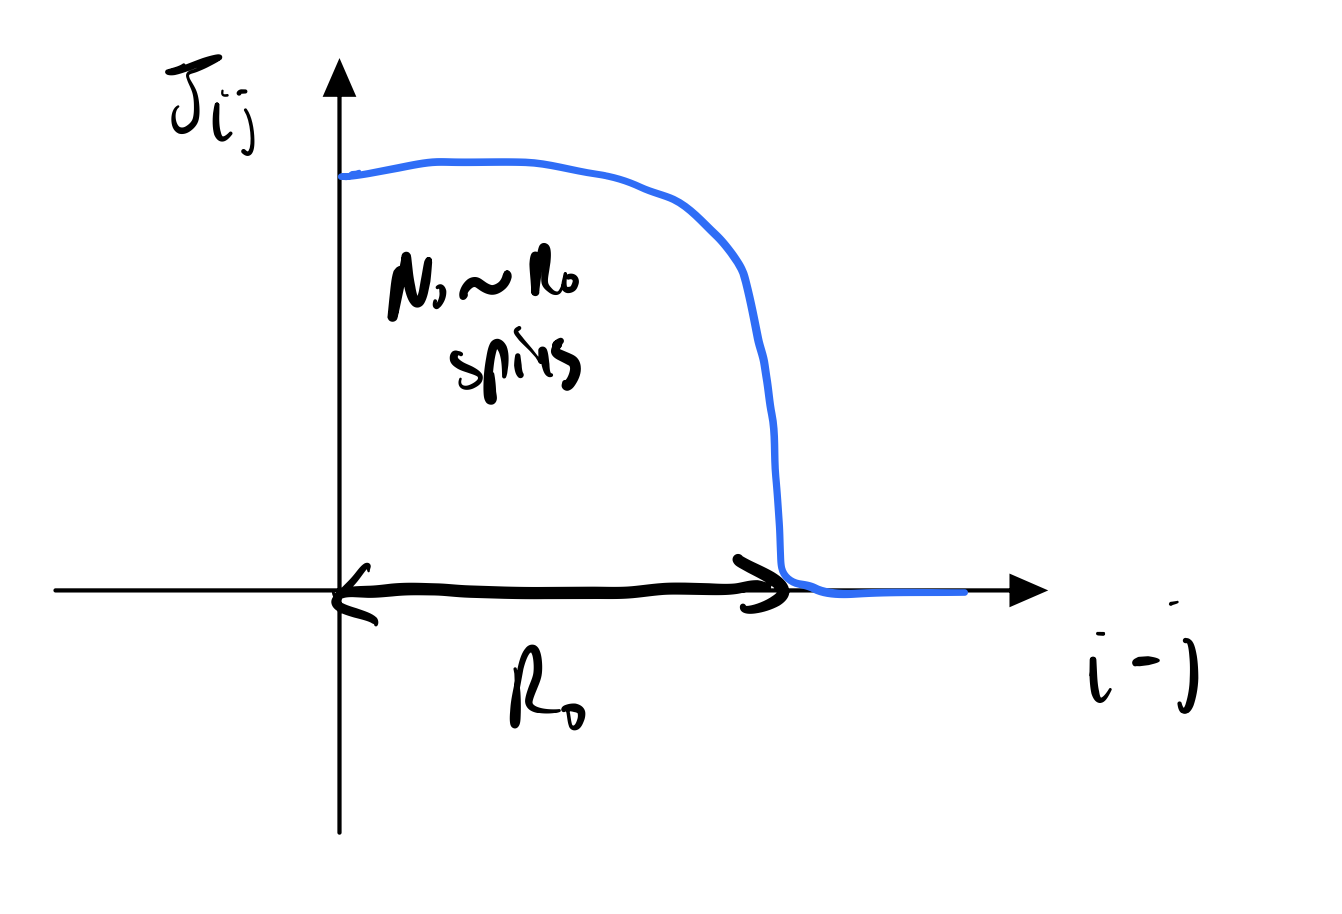
\includegraphics[scale=0.5]{Lectures/Figures/finite_range_interactions.png}
    \caption{Plot of the interactions/couplings $J_{ij}$, where the interactions are the same up to some long length scale $R_0$.}
    \label{fig:finite_range_interactions}
\end{figure}

In the Ising model, this looks like:
\begin{equation}
    H = \sum_{ij}JS_iS_j = \frac{J}{N_0}\sum_{\abs{i-j} < R_0}S_iS_j
\end{equation}
This looks like a coarse grained version:
\begin{equation}
    H = \sum_i S_i h_i
\end{equation}
where:
\begin{equation}
    h_i = \frac{J_0}{N_0}\sum_i S_i = J_0\avg{S}
\end{equation}
In the $N_0 \to \infty$ limit, this theory becomes correct (i.e. long range interactions get us closer to mean field theory, which makes sense! If all spins interact with each other, then the mean field literally is the physical field felt). A variant of this was used to win the Nobel prize last week (We will discuss the Hopfield model later in the course - it is a ferromagnet).

Note that the saddle point approximation works in a high number of dimensions, but it generally fails in a small number of dimensions - despite the dominance of the saddle point, there are many ways of making fluctuations; hence entropy comes in, competing with the energetics argument we have made here.

\subsection{Fluctuations}
We have two classes of models we consider, characterized by their symmetries.

\subsubsection*{Continuous (Rotational) Symmetries}
These are found, e.g., in X-Y models, Heisenberg models, superconductors. These generically have symmetries like $U(1), O(2), SO(2)$. The order parameters have amplitude and a phase, $\psi(x) = \abs{\psi_0}e^{i\theta(x)}$. At the mean field level, we can write $\abs{\nabla m}^2 = m_0^2 \abs{\nabla \Theta}^2$. We consider Hamiltonians with fluctuations of the form:
\begin{equation}
    \beta H = \text{Const} + \int d^d x\{\frac{1}{2}k\abs{\nabla\psi}^2\} \to \abs{\psi_0}^2\int d^dx \frac{1}{2}k(\nabla \Theta)^2 
\end{equation}
The stiffness is $\frac{1}{2}k\abs{\psi_0}^2$, where $\psi_0$ is the order parameter. Because this vanishes above the transition, the modes do not have stiffness above the critical point; they do below, with the stiffness vanishing as they approach the critical temperature. We can rewrite this as:
\begin{equation}
    \frac{1}{2}\abs{\psi_0}^2k\sum_a a \abs{\Theta_a}^2
\end{equation}
If we start populating these modes (as if they are bosons), we can get a very large number of them. We saw this in the AFM spin chain. Something similar will happen here. 

Why are they called soft modes? If I am far below $T_c$, the slope inb the dispersion relation is finite. As I approach $T_c$ in the mean field model, the slope goes to zero as the order parameters go to zero. Hence, they are ``soft''.

\begin{figure}[htbp]
    \centering
    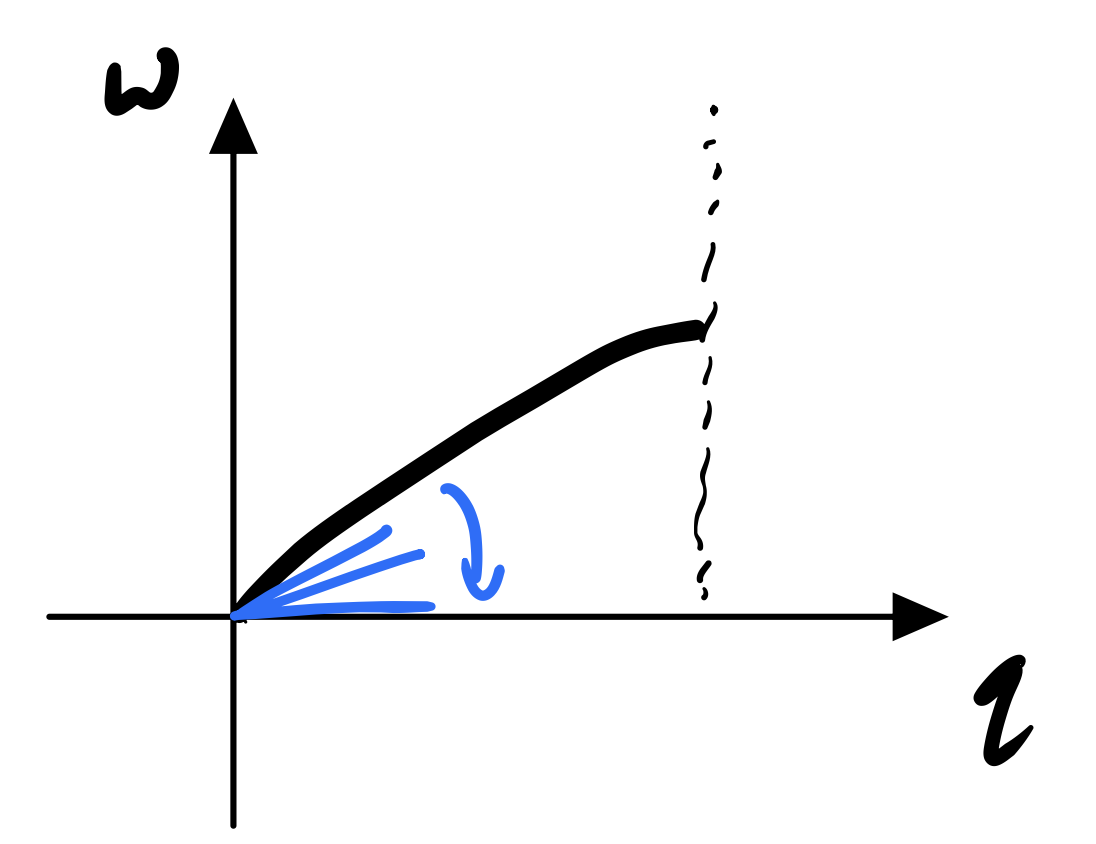
\includegraphics[scale=0.4]{Lectures/Figures/soft_modes.png}
    \caption{Depiction of ``soft modes'' in the dispersion relation, where as the temperature approaches the critical temperature below the slope in the dispersion (and the ``stiffness'') approaches zero.}
    \label{fig:soft_modes}
\end{figure}

\subsubsection*{Discrete ($\ZZ_2$) symmetry}
Next, we consider;
\begin{equation}
    \beta H = \int d^dx[\phi = \frac{1}{2}tm^2 + \frac{1}{4}um^4 + \frac{1}{2}k(\nabla m)^2]
\end{equation}
To which we can consider a more general E-L equation to find the extremum:
\begin{equation}
    k\nabla^2 m = tm + um^3
\end{equation}
We can now consider solutions that start into one well and cross into another well. We can solve this explicitly:
\begin{equation}
    m = m_0\tanh(\frac{x-x_0}{\omega})
\end{equation}
where the width is:
\begin{equation}
    \omega = \sqrt{\frac{2k}{-t}}
\end{equation}
This is another stationary solution; we previously found the lowest energy solution, this is a higher-lying stationary solution. As $t \to 0$, the domain wall becomes very long and the energy goes to zero. Notably, this is a particle-like excitation, with a lot of degrees of freedom as there are many points where it could be placed. Thus, we have to sum over all possible places to put 1, 2, \dots, $N$ domain walls. Each one has finite/small energy, but there are very many of these, so the entropic contribution is likely to win.

Next class, we will discuss how to measure these fluctuations (i.e. scattering experiments).